\section{Mô hình XGBoost}

\subsection{Giới thiệu}
Trong nghiên cứu này, mô hình XGBoost (Extreme Gradient Boosting) đã được triển khai nhằm dự đoán nồng độ khí CO (Carbon Monoxide) trong không khí dựa trên nhiều thông số môi trường như nhiệt độ, độ ẩm, áp suất không khí, và các chất ô nhiễm khác. XGBoost là một kỹ thuật học máy tiên tiến thuộc nhóm Ensemble Learning, nổi bật nhờ khả năng kết hợp hiệu quả nhiều cây quyết định (decision trees) thông qua phương pháp boosting. Mỗi cây trong mô hình được xây dựng tuần tự, nhằm sửa chữa những sai sót của cây trước đó, từ đó nâng cao độ chính xác tổng thể. Nhờ cơ chế tối ưu hóa gradient một cách mạnh mẽ, XGBoost không chỉ cải thiện hiệu suất dự đoán mà còn kiểm soát tốt hiện tượng overfitting, giúp mô hình hoạt động ổn định trên cả tập dữ liệu huấn luyện và kiểm thử.

\subsection{Tiền xử lý dữ liệu}
\begin{itemize}
    \item Loại bỏ các cột không cần thiết: chỉ giữ lại thông số CO(GT) chuẩn cũng như các thuộc tính dùng để dự đoán nồng độ CO(GT) đó như thông số về môi trường (nhiệt độ, độ ẩm, áp suất) và các thông số của các chất ô nhiễm đo được từ thiết bị đa cảm biến. 
    \item Xử lý giá trị thiếu (được ký hiệu là -200 trong dữ liệu): thay thế giá trị thiếu trong các cột bằng giá trị trước đó - cách xử lý thường dùng đối với dữ liệu dạng streaming như thế này.
    \item Xử lý giá trị ngoại lai: thay thế giá trị ngoại lai trong các cột bằng giá trị trước đó - cách xử lý thường dùng đối với dữ liệu dạng streaming như thế này.
    \item Xử lý các thuộc tính về thời gian: tách thuộc tính Date và Time thành các cột Year, Month, Day, Hour và xóa thuộc tính Date và Time.
\end{itemize}

\subsection{EDA}
\begin{itemize}
    \item Kiểm tra các thông tin cơ bản của dữ liệu: số hàng, số cột, kiểu dữ liệu của mỗi thuộc tính...
    \item Kiểm tra các thông tin thống kê của dữ liệu: trung bình, độ lệch chuẩn, các khoảng phân vị, min, max...
    \item Vẽ các biểu đồ để nắm thông tin về dữ liệu: 
    \begin{itemize}
        \item Area Charts: kiểm tra sự dao động của nồng độ các chất khí và các thông số môi trường (nhiệt độ, độ ẩm, áp suất) qua thời gian. 
        \item KDE Plots: kiểm tra sự phân phối của nồng độ các chất khí và các thông số môi trường (nhiệt độ, độ ẩm, áp suất). 
        \item Scatter Plots: kiểm tra mối liên hệ giữa nồng độ CO(GT) chuẩn với các thuộc tính còn lại. 
        \item Heatmap: kiểm tra hệ số tương quan giữa nồng độ các chất khí với nhau và với các thông số môi trường (nhiệt độ, độ ẩm, áp suất). 
    \end{itemize}
\end{itemize}

\subsection{Kiến trúc Mô hình XGBoost}

\subsubsection{Quy trình Huấn luyện}
\begin{enumerate}
    \item Tiến hành loại bỏ tiếp các thuộc tính không cần thiết tới CO(GT) dựa vào Heatmap có được từ bước EDA. 
    \item Tách thuộc tính phụ thuộc - CO(GT) với các thuộc tính độc lập. 
    \item Chia dữ liệu thành tập huấn luyện (80\%) và tập kiểm tra (20\%).
    \item Chuẩn hóa dữ liệu sử dụng MinMaxScaler.
    \item Huấn luyện mô hình trên tập huấn luyện.
    \item Đánh giá hiệu suất trên tập kiểm tra.
\end{enumerate}

\subsubsection{Tham số Mô hình}
Mô hình được triển khai với các tham số tối ưu:
\begin{itemize}
    \item \texttt{n\_estimators}: 100 cây quyết định.
    \item \texttt{learning\_rate}: tốc độ học của mỗi cây là 0.05. 
    \item \texttt{max\_depth}: độ sâu giới hạn của mỗi cây. 
    \item \texttt{subsample}: mẫu được chọn ngẫu nhiên từ 80\% dữ liệu gốc.
    \item \texttt{colsample\_bytree}: số thuộc tính được chọn ngẫu nhiên ở mỗi cây bằng 80\% số thuộc tính gốc. 
    \item \texttt{random\_state}: 42 để đảm bảo khả năng tái lập kết quả.
\end{itemize}

\subsection{Kết quả và Đánh giá}

\subsubsection{Các chỉ số Đánh giá}
Mô hình được đánh giá dựa trên các chỉ số:
\begin{itemize}
    \item Mean Squared Error (MSE) = 0.0133.
    \item Root Mean Squared Error (RMSE) = 0.1154.
    \item Mean Absolute Error (MAE) = 0.0764.
    \item R-squared (R²) = 0.7524.
\end{itemize}

\subsubsection{Trực quan hóa Kết quả}
Các biểu đồ được tạo ra để phân tích kết quả:
\begin{itemize}
    \item Biểu đồ so sánh giá trị thực tế và dự đoán:
    \begin{figure}[h]
        \centering
        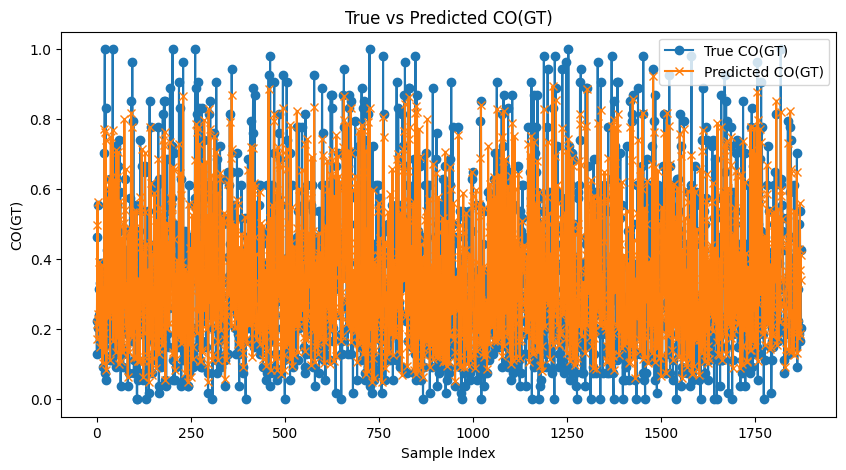
\includegraphics[width=0.8\textwidth]{images/xgboost/xgboost_true&predict.png}
        \caption{So sánh giá trị thực tế và dự đoán}
        \label{fig:xgboost_predictions}
    \end{figure}
    
    \item Biểu đồ phân tích phần dư:
    \begin{figure}[h]
        \centering
        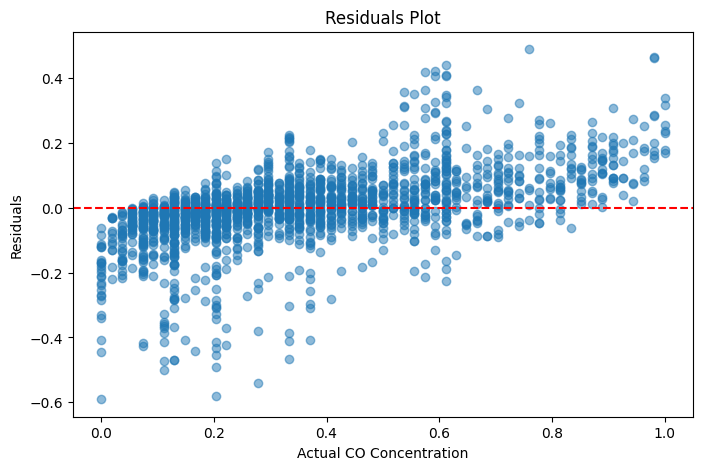
\includegraphics[width=0.8\textwidth]{images/xgboost/xgboost_residuals.png}
        \caption{Phân tích phần dư}
        \label{fig:xgboost_residuals}
    \end{figure}
\end{itemize}

\subsection{Kết luận}
Mô hình XGBoost đã dự đoán khá tốt giá trị nồng độ CO, thể hiện ở các chỉ số sai số khá tốt. Tuy nhiên, dựa vào biểu đồ phân tích phần dư, có thể thấy mô hình chỉ làm việc tốt khi nồng độ CO ở mức trung bình, điều này có thể xuất phát từ việc dữ liệu chưa đủ lớn ở các mốc ngoài mức trung bình, hoặc mô hình chưa thể học được các thông tin ẩn bên dưới...